\begin{figure}[htb]
	\centering
	\begin{subfigure}[t]{0.49\columnwidth}
		\centering
		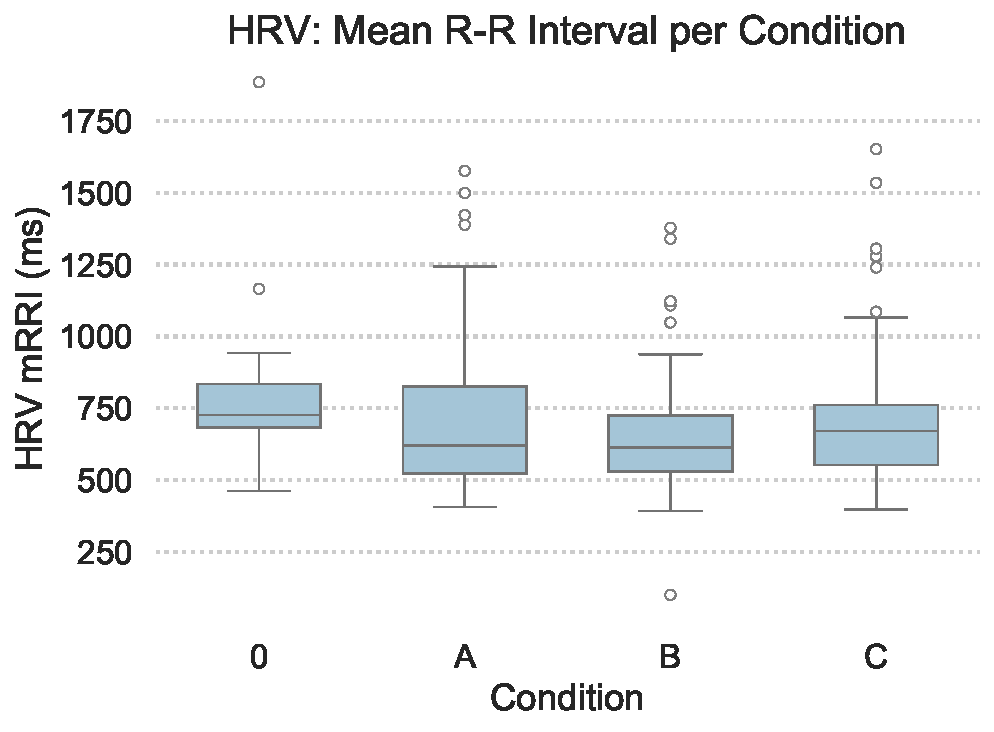
\includegraphics[width=\textwidth]{include/images/hrv_per_condition.pdf}
		\caption{\Glsfirst{mRRI} measured before (0) and during the conditions (A, B, and C) based on \gls{ECG}}
		\label{fig:stress-hrv}
	\end{subfigure}
	\hspace*{\fill}
	\begin{subfigure}[t]{0.49\columnwidth}
		\centering
		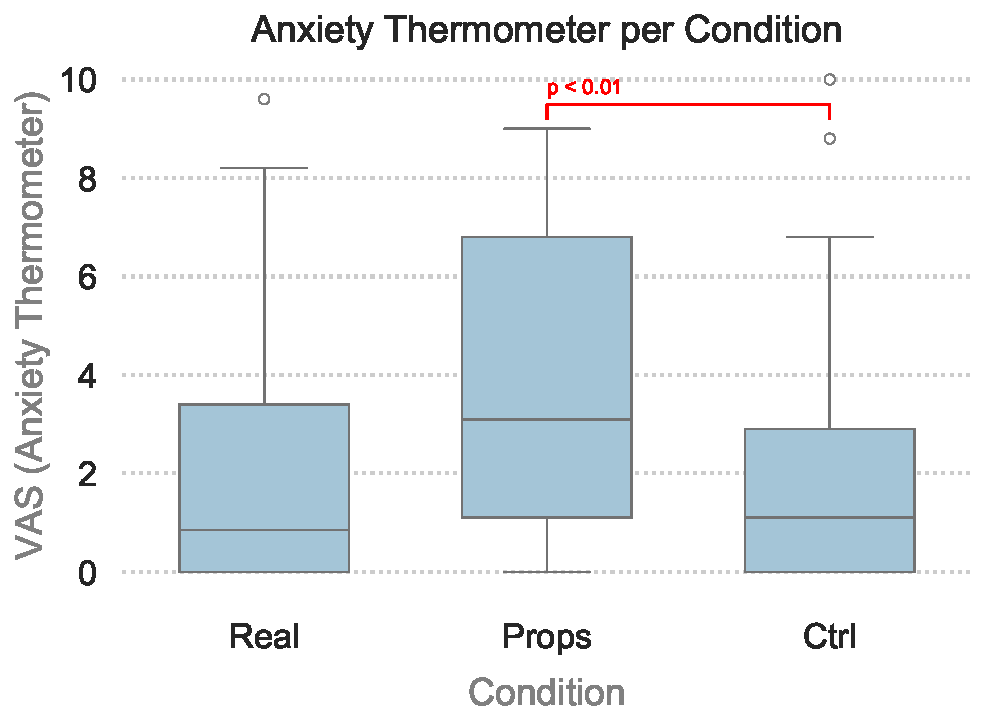
\includegraphics[width=\textwidth]{include/images/at_per_condition.pdf}
		\caption{Average anxiety as reported via \glsfirst{VAS} after each condition (A, B, and C) on a scale from 0 to 10}
		\label{fig:anxiety-at}
	\end{subfigure}
	\captionsetup{subrefformat=parens}
	\caption[Results: stress and anxiety]{Results for stress and anxiety, measured with \gls{HRV} \subref{fig:stress-hrv}, and by self report \subref{fig:anxiety-at}}
	\label{fig:stress-anxiety}
\end{figure}